
Transformers are predominantly utilized in generating text for Large Language Models (LLMs) like GPT \autocite{GPT2radford2019} and LaMMA \autocite{touvron2023llama}. This thesis aims to explore the application of conventional Transformer-based architectures for the generation of texture assets, diverging from the traditional image generation methods primarily relying on stable diffusion techniques or Generative Adversarial Networks (GANs).

To achieve this, three distinct models are developed and trained, each incorporating unique modifications to harness the principal benefits of Transformer-based models for image texture generation. The dataset required for training these models is compiled from a variety of sources, necessitating thorough cleaning and analysis to ensure usability. The objective is for these trained models to be capable of generating basic floor textures suitable for use as assets in video games. These developed models are compared using a specific set of metrics. Furthermore, the development process will be briefly outlined, highlighting the differences from conventional programming workflows typically encountered.



\subsection{Related work}
    
The exploration of machine learning models for image generation has been a significant area of research lately, with notable advancements from Generative Adversarial Networks (GANs) to state-of-the-art diffusion models. This section reviews the seminal works and recent innovations in the field, particularly focusing on image/texture generation and the application of Transformer models in the context of images, laying the foundation for the current study's approach to image generating.

\textbf{Generative Adversarial Networks (GANs):} 
Since their introduction by \autocite{goodfellow2014generative}, GANs have been a cornerstone in the field of generative models, especially for image generation tasks. Works by \autocite{radford2016unsupervised}, introducing the DCGAN architecture, demonstrated the potential of GANs in producing high-quality images. The adaptability of GANs has been explored in various contexts, including texture synthesis \autocite{xian2018texturegan}, showcasing their capability to generate seamless textures for different materials.

\textbf{Diffusion Models:} 
Diffusion models represent a cutting-edge development in the field of generative models, that demonstrate remarkable capabilities in image generation by iterative denoising a random signal to produce detailed images. The process, initially introduced by \autocite{sohldickstein2015deep}, involves gradually adding noise to an image across several steps and then learning to reverse this process. Stable diffusion, a term often associated with these models, refers to the technique's ability to maintain stability throughout the noise addition and removal process, ensuring high-quality image synthesis. The paper \enquote{Diffusion Models Beat GANs on Image Synthesis} \autocite{dhariwal2021diffusion} further refined this concept with models like DDPM, showcasing exceptional fidelity in generated images. This approach contrasts traditional models by focusing on the controlled removal of noise, leading to the generation of coherent and visually impressive images.

\textbf{Transformers in Image classification:} 
The success of Transformer models in natural language processing, as seen with architectures like GPT \autocite{GPT2radford2019} and LaMMA \autocite{touvron2023llama}, has inspired their application in image-related tasks. The Vision Transformer (ViT) by \autocite{dosovitskiy2021image} marked a significant leap, applying Transformers directly to sequences of image patches for classification tasks. This idea was extended to image generation through architectures like the VideoGPT by \autocite{yan2021videogpt}, which demonstrated that Transformer models could generate coherent and detailed videos.

\textbf{Texture Generation with Transformers:}
TransGAN by \autocite{jiang2021transgan} revolutionizes image generation with a Transformer-based GAN architecture, moving beyond traditional CNN approaches. It features a memory-efficient generator and a nuanced, multiscale discriminator, both utilizing transformer blocks. With advanced training techniques to overcome common GAN challenges, TransGAN produces high-quality images, showcasing the potential of Transformers in this new domain.

\subsection{Infrastructure for Model Development}

To develop and train the models in this thesis, a powerful computing infrastructure is necessary to manage the extensive datasets and the substantial computational requirements for model training. Unlike conventional development environments where a standard laptop or desktop may suffice, most of the models in this thesis demand a more capable infrastructure. Therefore, a high-performance computing system situated in Berlin is used for the model training processes. This system contains an array of (NVIDIA Tesla A100 80 GB) GPUs, (INTEL Ice Lake 8360Y) CPUs and a significant quantity of RAM. Such a configuration, especially the substantial GPU memory, enables the training and execution of larger models that would be possible on a home workstation. The development of these models is carried out using Python and PyTorch, with the code being crafted in Visual Studio Code and managed through version control with Git. The model development and initial code testing are done on a local machine, reserving the high-performance system exclusively for the final training phases. This approach diverges from standard practices, where often both development and execution occur on the same development platform. Ensuring the code is free of errors prior to giving the task of training the model to the high-performance computing system is crucial, as discovering bugs in the training process can be exceedingly time-consuming. For instance, to endure a training session that extends for 30 hours, only to realize it terminated prematurely due to script errors.

\subsection{Data}
    
This section describes the methods used for gathering, cleaning, and analyzing data for this thesis. Essential for training a machine learning model, the data is carefully collected from various sources, cleaned to maintain uniformity, and examined for patterns, with a focus on color distribution.


\subsubsection{Data Retrieval}
On the internet, a wide variety of textures can be found, but not all of them are suitable for this task. The textures should be seamless, devoid of shadows, and free from any objects. Textures of floors, such as carpets, tiles, wood, concrete, and more, were utilized. Two approaches were employed to acquire the data for this thesis.

\begin{itemize}
    \item Web Data Collection

    Some data for this project was obtained from various online sources. Numerous free texture providers were utilized for data acquisition. Due to the limitation of downloading one texture at a time from most websites, a series of scripts were developed to compile a list of suitable textures and automate the downloading process. These scripts were created using UiPath and Python.
    
    \item Video Game Textures

    The second approach involved using textures from video games. The advantage of this approach is that it allows for the acquisition of many textures simultaneously. However, a drawback is that these collections of textures include normal maps, height maps, and many other assets that are not suitable.


\end{itemize}

\subsubsection{Data Cleaning}

    To ensure that the data is consistent and free from elements that could corrupt the model, various cleaning steps were applied. For example, all images containing 3D objects were removed. To obtain the cleaned textures from the video game sources, a Python script is used to discard images containing certain keywords like `\_no.png', `\_spec.png', and many others. Additionally, an image should contain a keyword like `floor', `wall', `wood', or `stone'. In summary, 129 good keywords and 56 bad keywords were utilized. The major challenge with this approach is that you can't filter with 100\% accuracy, so all the textures are manually checked. In addition, some textures are only usable as overlays for 3D models and aren't supposed to be flat 2D images on their own. So, these are also filtered out. In total, only 20-30\% of textures from a video game are viable for use in this thesis.

    In the case of web-gathered textures, the textures are often in different folder structures, and it was necessary to standardize them across all data folders. Additionally, some of them had associated files that were irrelevant to this use case and needed to be discarded.

    Finally, the images are cropped to 512x512 or 1024x1024 pixels, as these are the sizes used in this thesis. In total, 57454 images of size 512x512 were collected and 12600 being of size 1024x1024 pixels. The sources are summarized in \autoref{tab:datasets}.

    \begin{table}[H]
        \centering
        \begin{adjustbox}{width=0.8\textwidth}
          \begin{tabular}{|r|c|r|r|}
              \hline
              Source & Type & Number of Images [size 512x512] & Number of Images [size 1024x1024] \\
              \hline
              0 & Game assets & 56 & 14 \\
              1 & Game assets & 3,236 & 809 \\
              2 & Game assets & 2,152 & 539 \\
              3 & Game assets & 184 & 46 \\
              4 & Game assets & 1808 & 452 \\
              5 & Game assets & 100 & 25 \\
              6 & Game assets & 309 & 71 \\
              7 & Game assets & 4154 & 809 \\
              8 & Game assets & 16 & 4 \\
              9 & Game assets & 1,084 & 271 \\
              10 & Website & 1,052 & 263 \\
              11 & Game assets & 102 & 20 \\
              12 & Game assets & 1,334 & 36 \\
              13 & Game assets & 409 & 24 \\
              14 & Game assets & 76 & 19 \\
              15 & Game assets & 5,789 & 628 \\
              16 & Game assets & 632 & 158 \\
              17 & Game assets & 1 & --- \\
              18 & Game assets & 1,984 & 491 \\
              19 & Website & 196 & 49 \\
              20 & Website & 1,756 & 439 \\
              21 & Game assets & 643 & 110 \\
              22 & Game assets & 69 & --- \\
              23 & Game assets & 1,656 & 414 \\
              24 & Game assets & 4,188 & 1,047 \\
              25 & Game assets & 24 & 6 \\
              26 & Game assets & 2,980 & 745 \\
              27 & Game assets & 996 & 14 \\
              28 & Game assets & 492 & 123 \\
              29 & Game assets & 2,096 & 524 \\
              30 & Website & 17,816 & 4,434 \\
              31 & Game assets & 8 & 2 \\
              32 & Game assets & 4 & 1 \\
              33 & Game assets & 52 & 13 \\
              \hline
              Total & Game assets & 36,634 & 7,415 \\
                    & Website & 20,820 & 5,185 \\
              \hline
              Total & & 57,454 & 12,600 \\
              \hline
          \end{tabular}
        \end{adjustbox}
        \caption{The Dataset collected for this thesis}
        \label{tab:datasets}
    \end{table}

    \subsubsection{Patterns in the data}
    
    To examine whether the dataset encompasses a broad spectrum of colors, multiple plots are created. These plots illustrate the color distribution within the datasets, providing insights into the diversity of colors present. Prior to plotting, a comprehensive pixel count across all images is conducted. For instance, if an image features 10 pixels of the color $(255, 0, 0)$, this count is added to a dictionary. Should the subsequent image in the dataset contain 5 pixels of the same color, these are also incorporated into the dictionary, cumulating a total of 15 for that specific color. This process is repeated for each color encountered, aggregating the counts to yield the overall color frequency within the dataset.

\begin{lstlisting}[language=Python]
  color_counts = {} 
  for i, (data, _) in enumerate(dataset):
      # data is a tensor of shape (3, height, width) 
      pixel_rgb_array = (data.view(3, -1).t() * 255).to(torch.int32)
      
      for pixel_color in map(tuple, pixel_rgb_array):
          if color in color_counts:
              color_counts[pixel_color] += 1
          else:
              color_counts[pixel_color] = 1
\end{lstlisting}

    After analyzing the dataset through this method, visual representations of the color distributions were produced using Python, Seaborn and Matplotlib. 
    
    \subsubsection{Data Lab plots}

    The following plot illustrates the color distributions of the whole dataset in the lab color spectrum.


    \begin{figure}[H]
        \centering
        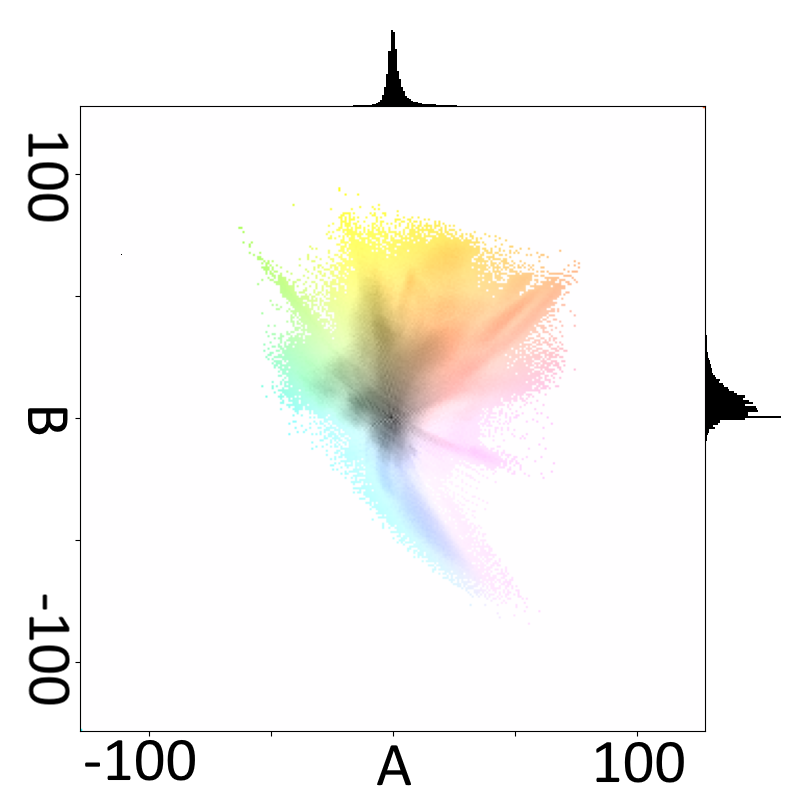
\includegraphics[width=0.8\textwidth]{../code/dataAnalysis/plots/lab/labPlot_1.png}
        \caption{Color distribution of the dataset in the LAB color space}
        \label{fig:example}
    \end{figure}
    
    This visualization primarily consists of a central plot complemented by two histograms on its top and right sides. The central plot is a color map representing the distribution of colors from the original data in the CIELAB (Lab) color space, specifically focusing on the 'a' and 'b' components. The 'a' axis (horizontal) indicates the position between green and red colors, while the 'b' axis (vertical) shows the position between blue and yellow colors.

    The color map itself is constructed by converting Lab color values back into the RGB color space for display. Colors are distributed across this plot based on their 'a' and 'b' values, with the lightness ('L' component of Lab) squeezed into the 2D plane. The areas with no data are shown in white.

    The histograms on the top and right sides of the central plot provide additional context by showing the distribution of 'a' and 'b' values across the dataset. They are weighted by a logarithmic transformation of the count of colors. This logarithmic scaling helps in highlighting patterns in the data without allowing very high or very low counts to dominate the visualization.

    The plot demonstrates that the dataset encompasses a broad array of colors, with a significant quantity of colors spread throughout the entire spectrum. However, the histograms on the sides suggest that the dataset primarily consists of colors in the middle of the spectrum, indicating that it is not overly colorful but leans more toward the white/gray/black spectrum. This could be attributed to the fact that most of the textures are floor textures, which are typically not very colorful. All the various sources are presented as a lab plot in the appendix; see \autoref{sec:app_labPlots}.

    \subsubsection{Data RGB plots}

    The second plots provide a three-dimensional view of the RGB color space, where the X, Y, and Z axes correspond to the Red, Green, and Blue color values, respectively, each ranging from 0 to 255. 

    \[
    \text{size} = \log(\text{count of color}) \times 20
    \]

    The size of each plotted point is determined by the logarithm of the color count, scaled by a factor of 20. See \autoref{fig:rgb_all} for the combined color distribution of all sources. There, it is also clearly visible that most of the sources are not very colorful, leaning more towards the white/gray/black color spectrum.

    \subsubsection{Data Synchronization}

    In the thesis, a manual data synchronization routine is established to maintain data consistency between the supercomputer located in Berlin and the local workstation.

\subsection{Models}
    (LLMs, basic idea, roll model, spiral model)

    \subsubsection{Large Language Models (LLMs)}

    Large Language Models (LLMs) are a class of machine learning models that have gained significant attention in recent years due to their ability to generate coherent and contextually relevant text. These models are trained on vast amounts of text data, enabling them to understand and generate human-like text. The GPT models by OpenAI \autocite{GPT2radford2019} is a prominent example of an LLM, capable of generating human-like text and performing a wide range of language-related tasks. Like LLMs, the models developed in this thesis predict the next thing in a sequence. But instead of predicting the next word in a sentence, they predict the next pixel in an image. This is achieved by treating the image as a sequence of pixels and using the transformer architecture to predict the next pixel in the sequence.

    \subsubsection{Adapting Transformer Architecture for Image Prediction}

    The Transformer architecture, introduced by \autocite{vaswani2023attention}, has significantly impacted the field of natural language processing (NLP). Its widespread adoption across a variety of language tasks, such as machine translation and text generation, highlights its transformative influence. At the heart of the Transformer's success is the self-attention mechanism, which allows the model to weigh different portions of the input data dynamically. This critical feature enables the detection of long-range dependencies and a deeper understanding of the context within the input, making the architecture highly effective for complex NLP tasks.

    Building upon this foundation, this thesis explores the extension of the Transformer architecture from its traditional role in NLP to the domain of image prediction. This adaptation employs the architecture's fundamental principles, especially the self-attention mechanism. By treating images as sequences of pixels, the Transformer architecture is applied to predict subsequent pixels in an image sequence, showcasing its potential versatility beyond text-based applications.
    
    \subsubsection{Column Image Transformer}

    In the context of this thesis, a model termed the Column Image Transformer (CIT) has been conceptualized and developed. This model embodies an adaptation of the conventional transformer architecture. Distinctively, the CIT model diverges from traditional image processing techniques by segmenting the image into vertical slices or columns of pixels. This segmentation allows for a method where each column is processed on its own, following the "B" batch dimension in the model's structure.

    The adaptation of self-attention for image prediction involves sequentially processing the image, similar to text in natural language processing. However, instead of words or characters, the sequence consists of pixels. In the Column Image Transformer (CIT) model, the image is divided into columns, and the self-attention mechanism is applied to understand the relationships between pixels within each column. This should enable the model to predict the properties of subsequent pixels in a column by considering the context provided by preceding pixels.

    \subsubsection{Spiral Image Transformer}

    The second approach is represented by the Spiral Image Transformer (SIT). Unlike its predecessor, the Column Image Transformer (CIT), the SIT model employs a contextually spiral pattern. This architecture enables the generation of images starting from a central point and expanding outward (see ...). In the SIT model, the batch dimensions correspond to distinct images, whereas the H dimension represents the spiral context. Similar to the CIT model, the C dimension denotes the color channels.

    One of the pivotal enhancements of the SIT model is its ability to analyze adjacent pixels on the horizontal axis, in contrast to the CIT model's limitation to columnar pixel analysis. This feature is particularly beneficial for interpreting textures with intricate patterns, such as diagonal ones, thereby offering an advantage over the Column Image Transformer. However, it is important to note that the SIT model operates within a constrained area of the image due to its 2D context. This limitation necessitates the use of only a portion of the image area, specifically a sector determined by the square root of the total area available to the Column Image Transformer (CIT), with an equal context length.
    
    In the Spiral Image Transformer (SIT) model, the self-attention mechanism is adapted to analyze pixels in a spiral pattern. This approach allows the model to evaluate the context in a manner that incorporates both the immediate neighborhood and the broader context of the image, facilitating the prediction of pixel properties in a way that captures complex, two-directional patterns and textures. The self-attention mechanism's ability to dynamically focus on different parts of the spiral sequence should enable these models to generate coherent predictions for the next pixel, based on the learned importance of each pixel to the others.
